\documentclass[12pt]{article}
%Also I made it 12pt

\usepackage[fontset=macnew]{ctex}
\usepackage{physics}
\usepackage{tikz}
\usetikzlibrary{3d,calc,patterns}
% \usepackage{tkz-euclide}
\usepackage{amsmath}
\usepackage{mathrsfs}
\usepackage{upgreek}
\usepackage{amsthm}
\usepackage{amsfonts}
%to add an affiliation line to the the title formatting
\usepackage{authblk}

%Fonts
% \usepackage[no-math]{fontspec} %This allows you to enter (via an IPA kayboard) IPA fonts and other symbols directly into LaTeX. Requires a particular setyp, see below.
\usepackage{libertine} %A font that actually contains many IPA symbols. This is the font you see in the preview to the right.

%to use these fonts, be sure that your typesetting engine is set to "XeLaTeX." In Overleaf, go to the Menu link on the top left (by the Overleaf icon), and under Settings be sure that the Compiler is set to "XeLaTeX." If you accessed this document via the Overleaf Pomona Linguistics template, all of this was already done for you.

%The Pomona Linguistics Paper Template in Overleaf is already set up for this, but you may run into this problem if you start building your own documents.


%%%%%%%%%%%%%%%%%%%%%%%%%%%%%%%%%%%%%%%%%%%%%%%%%%%
%packages for this style of handout-formatting of (sub)section headers 
\usepackage[explicit]{titlesec}
\usepackage{xcolor}

\definecolor{light-gray}{gray}{0.7}
\definecolor{lighter-gray}{gray}{0.85}

\titleformat{\section}
{\normalfont\Large\bfseries}{}{0em}{\colorbox{black}{\parbox{\dimexpr\textwidth-2\fboxsep\relax}{\textcolor{white}{\thesection\quad#1}}}}

\titleformat{\subsection}
{\normalfont\large\bfseries\scshape}{}{0em}{\colorbox{light-gray}{\parbox{\dimexpr\textwidth-2\fboxsep\relax}{\textcolor{black}{\thesubsection\quad#1}}}}

\titleformat{\subsubsection}
{\normalfont\bfseries}{}{0em}{\colorbox{lighter-gray}{\parbox{\dimexpr\textwidth-2\fboxsep\relax}{\textcolor{black}{\thesubsubsection\quad#1}}}}
%%%%%%%%%%%%%%%%%%%%%%%%%%%%%%%%%%%%%%%%%%%%%%%%%%%

%%% This file is the preamble for the Pomona Linguistics LaTeX Paper Template, which is also used for the Quick Reference Guide. If you are brand new to writing with LaTeX, we suggest NOT messing with it, and just writing your paper using the Paper Template. If you are getting more comfortable in LaTeX and want to add packages and commands, this is where you do it (when using this template).

%For stacking text, used here in autosegmental diagrams
\usepackage{stackengine}

%To combine rows in tables
\usepackage{multirow}

%geometry helps manage margins, among other things.
\usepackage[margin=1in]{geometry}

%Gives some extra formatting options, e.g. underlining/strikeout
\usepackage{ulem}

%For putting links into papers, also helps make cross-references in the paper smart references
\usepackage[colorlinks = true,
            linkcolor = blue,
            urlcolor  = blue,
            citecolor = blue,
            anchorcolor = blue]{hyperref} %smarter cross-references, these options turn links blue

%Use package/command below to create a double-spaced document, if you want one. Uncomment BOTH the package and the command (\doublespacing) to create a doublespaced document, or leave them as is to have a single-spaced document.
%\usepackage{setspace}
%\doublespacing 

%paragraph formatting
\usepackage[parfill]{parskip}
\setlength{\parskip}{5pt} %plus 1 minus 1}
\setlength{\parindent}{30pt}
\usepackage{titlesec}

%use for special OT tableaux symbols like bomb and sad face. must be loaded early on because it doesn't play well with some other packages
\usepackage{fourier-orns}

%Basic math symbols 
\usepackage{pifont}
\usepackage{amssymb}

%%%Gives shortcuts for glossing. The use of this package is NOT explained in the Quick Reference Guide, but the documentation is on CTAN for those that are interested. MJKD finds it handy for glossing. (https://ctan.org/pkg/leipzig?lang=en)
\usepackage{leipzig}

%Tables
\usepackage{caption} %For table captions
\usepackage{booktabs} %helps format tables

%For citations and bibliography - as of 9.1.2019 we don't explain citations in this Quick Reference Guide, but Pedro Martin's tutorial does (see links in the Guide).
\usepackage{natbib}

%For OT-style tableaux
\usepackage{ot-tableau}

%highlights text with \hl{text}
\usepackage{color, soul}

%Drawing Syntax Trees
\usepackage[linguistics]{forest}

%This specifies some formatting for the forest trees to make them nicer to look at
\forestset{
  nice nodes/.style={
    for tree={
      inner sep=0pt,
      fit=band,
    },
  },
  default preamble=nice nodes,
}

%% For numbered and glossed examples %%
\usepackage{gb4e}



%Changes the \maketitle command to be smaller and take up less space on a page. 
\makeatletter         
\def\@maketitle{   % custom maketitle 
\noindent {\Large \bfseries \color{black} \@title}  \\ \hrule \noindent \@author \\ \@date  
}

%The code below will draw a circle around a piece of text. This is very useful for drawing attention to a word in a data example. use the command \circled{text} where the argument (`text' here) is what you want to be circled. This is illustrated in the Quick Reference Guide and the Paper Template.

\usepackage{tikz}

\newcommand{\circled}[1]{\begin{tikzpicture}[baseline=(word.base)]
\node[draw, rounded corners, text height=8pt, text depth=2pt, inner sep=2pt, outer sep=0pt, use as bounding box] (word) {#1};
\end{tikzpicture}
}


%%%%%%%%%%%%%%%%%%%%%%%%%%%%%%%%%%%%%%%%%%%%%%%%%%%%%%%%%%%%
%%%%%%%%%%%%%%%%%%%%%%%%%%%%%%%%%%%%%%%%%%%%%%%%%%%%%%%%%%%%

% Useful Ling Shortcuts

\RequirePackage{leipzig}
%\RequirePackage{mathtools} % for \mathrlap

% % % Shortcuts  (borrowed from JZ, I'm still unsure exactly what xspace requires)
\RequirePackage{xspace}
\xspaceaddexceptions{]\}}

%This makes the \emptyset command be a nicer one
\let\oldemptyset\emptyset
\let\emptyset\varnothing
\newcommand{\nothing}{$\emptyset$}

%Not all of these are explained in the Quick Reference Guide, but they are here bc they are relevant to some of our students.
\newcommand{\1}{\rlap{$'$}\xspace}
\newcommand{\0}{\rlap{\textsuperscript{$ˆ{\circ}$}}\xspace}
\newcommand{\Lb}[1]{$\text{[}_{\text{#1}}$ } %A more convenient left bracket
\newcommand{\Rb}[1]{$\text{]}_{\text{#1}}$ } %A more convenient left bracket
\newcommand{\gap}{\underline{\hspace{1.2em}}}
\newcommand{\vP}{\emph{v}P}
\newcommand{\lilv}{\emph{v}}
\newcommand{\Abar}{A$'$-} %A more convenient A-bar notation
\newcommand{\ph}{$\varphi$\xspace} %A more convenient phi
\newcommand{\pro}{\emph{pro}\xspace}
\newcommand{\subs}[1]{\textsubscript{#1}} %A more convenient subscript
%\newcommand{\hd}{$^{\circ}$\xspace} %Symbol for printing head / degree symbol
\newcommand{\spells}{$\Longleftrightarrow$} %spellout arrow for morph spellout rules
% \newcommand{\tr}[1]{\textit{t}\textsubscript{\textit{#1}}} %easy traces with subscript
\newcommand{\supers}[1]{\textsuperscript{#1}}

% Abbreviations for glossing, based on Leipzig
\newleipzig{hab}{hab}{habitual}
\newleipzig{rem}{rem}{remote}
\newleipzig{sm}{sm}{subject marker}
\newleipzig{t}{t}{tense}
\newleipzig{aa}{aa}{anti-agreement}
\newleipzig{pron}{pron}{pronoun}
\newleipzig{rec}{rec}{recent}
\newleipzig{om}{om}{object marker}
%\newleipzig{ipfv}{ipfv}{imperfective}
\newleipzig{asp}{asp}{aspect}
\newleipzig{lk}{lk}{linker}
\newleipzig{pcl}{pcl}{particle}
\newleipzig{stat}{stat}{stative}
\newleipzig{ints}{ints}{intensive}
\newleipzig{ascl}{ascl}{assertive subject clitic}
\newleipzig{nascl}{nascl}{non-assertive subject clitic}
\newleipzig{ta}{ta}{tense and/or aspect}
\newleipzig{assoc}{assoc}{associative marker}
\newleipzig{hon}{hon}{honorific}
%\newleipzig{whprt}{wh}{\wh particle}
\newleipzig{sa}{sa}{subject agreement}
\newleipzig{conj}{conj}{conjunction}
%\newleipzig{loc}{loc}{locative}
\newleipzig{expl}{expl}{expletive}
\newleipzig{rcm}{rcm}{reciprocal marker}
\newleipzig{pers}{pers}{persistive}
%\newleipzig{}{}{} %this is just to copy for when I want to add more

%%%%%%%%%%%%%%%%%%%%%%%%%%%%%%%%%%%%%%%%%%%%%%%%%%%%%%%%%%%%
%%%%%%%%%%%%%%%%%%%%%%%%%%%%%%%%%%%%%%%%%%%%%%%%%%%%%%%%%%%%

%A couple of packages that seemed to prefer being called toward the end of the preamble

%This package provides macros for typesetting SPE-style phonological rules.
\usepackage{phonrule}

%For using Greek letters outside of math mode.
\usepackage{textgreek}


%Random, lets us use the XeLaTeX logo. Not important to the template at all.
\usepackage{metalogo}


%%%%%%%%%%%%
%% This is the end of the PREAMBLE
%%%%%%%%%%%

%MJKD note to future self - this preamble is just the section headers + PomLing formatting, but an ordering paradox between the two files made me combine them and re-order fontspec. *shrug* In future if it needs an update, just take the PomLing formatting file and add in the section headers for handouts.

\newcommand{\rmd}{\mathrm{d}}
\newcommand{\deriv}[2]{\frac{\rmd #1}{\rmd #2}}
\newcommand{\pderiv}[2]{\frac{\partial #1}{\partial #2}}
\newcommand{\dpderiv}[2]{\dfrac{\partial #1}{\partial #2}}
\newcommand{\dderiv}[2]{\dfrac{\rmd #1}{\rmd #2}}

\title{真空中的恒定磁场}
\author{\href{mailto:lai-wei@whu.edu.cn}{Lai Wei}}
\date{\today}

\begin{document}

\maketitle

\section{恒定电流}

\subsection{电流 \quad 电流密度}

\begin{equation}
    \boldsymbol{j} = \deriv{I}{S_0} \boldsymbol{e}_{\text{n}}
\end{equation}

\begin{itemize}
    \item 方向:改点正电荷运动的方向,即$\boldsymbol{e}_{\text{n}}$;
    \item 大小:$j = \dderiv{I}{S_0} = \dderiv{I}{S \cos \theta}$。
\end{itemize}

通过面积元的电流为

\begin{equation}
    I = \int_S \boldsymbol{j} \cdot \rmd \boldsymbol{S}
\end{equation}

\subsection{电流的连续性方程 \quad 电路恒定的条件}

在导体内任取一封闭曲面$S$,由电荷守恒

\begin{equation}
    \oint_S \boldsymbol{j} \cdot \rmd \boldsymbol{S} = - \deriv{Q}{t}
\end{equation}

由$Q = \int_V \rho \rmd V$ ($\rho = \rho(x,y,z,t)$为电荷体密度分布函数),

\begin{equation}
    \oint_S \boldsymbol{j} \cdot \rmd \boldsymbol{S} = \int_V \pderiv{\rho}{t} \rmd V
\end{equation}

\subsection{欧姆定律及其微分形式}

由电阻定律,

\begin{equation}
    R = \rho \frac{l}{S}
\end{equation}

电流在不均匀的导体中流动:

\begin{equation}
    R = \int \rmd R = \int \rho \frac{\rmd l}{S}
\end{equation}

沿电场线方向,取长$\rmd l$、横截面积$\rmd S$的微流管,电阻率为$\rho$,则

\begin{equation}
    j = \frac{1}{\rho}\left(-\deriv{V}{l}\right) = \sigma E
\end{equation}

矢量形式为

\begin{equation}
    \boldsymbol{j} = \sigma \boldsymbol{E}
\end{equation}

\subsubsection{例题}

如图\ref{p12-1}所示,高度为\(h\)的两个共轴金属圆环,其内环的外半径和外环的内半径分别为\(R_1\)和\(R_2\)。两环间充满电阻率为\(\rho\)的均匀导电材料($\rho$4远大于金属圆环的电阻率)。
当圆环之间加上电压\(U\)后,电流沿径向由内向外流动。试求

\begin{enumerate}
    \item 两环之间导电材料的总电阻;
    \item 两环之间距离为\(r\)处电流密度的大小和方向。
\end{enumerate}

\begin{figure}[!h]
    \centering
    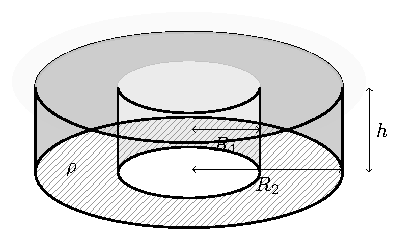
\includegraphics{graphics/p12.1.pdf}
    \caption{例题1}
    \label{p12-1}
\end{figure}

在导电材料上任取一半径为$r$,宽度为$\rmd r$,高度为$h$的薄圆环,其侧面积为$2 \uppi r h$,则薄圆环的径向电阻为

\begin{equation*}
    \rmd R = \rho \frac{\rmd r}{2 \uppi rh}
\end{equation*}

所以整个导电材料的径向总电阻为

\begin{equation*}
    R = \int \rmd R = \int_{R_1}^{R_2} \rho \frac{\rmd r}{2 \uppi rh} \ln \frac{R_2}{R_1}
\end{equation*}

由欧姆定律可得导电材料中的径向总电流为

\begin{equation*}
    I = \frac{U}{R} = \frac{2 \uppi h U}{\rho \ln(R_2/R_1)}
\end{equation*}

于是在距离环心为\(r\)处电流密度的大小为

\begin{equation*}
    j = \frac{I}{S} = \frac{I}{2 \uppi r h} = \frac{U}{r \rho \ln(R_2/R_1)}
\end{equation*}

\subsection{电源\quad 电动势}

电动势

\begin{equation}
    \mathscr{E} = \int_{-}^{+} \boldsymbol{E}_{\text{k}} \cdot \rmd l
\end{equation}

闭合回路的总电动势

\begin{equation}
    \mathscr{E} = \oint_L \boldsymbol{E}_{\text{k}} \cdot \rmd l
\end{equation}

\section{磁场 \quad 磁感应强度}

定义磁感应强度\(\boldsymbol{B}\)的大小为

\begin{equation}
    B = \frac{F_{\text{max}}}{qv}
\end{equation}

运动电荷在磁场中受到的磁场力可表示为

\begin{equation}
    \boldsymbol{F} = q \boldsymbol{v} \times \boldsymbol{B}
\end{equation}

这就是运动电荷在磁场中受到的磁场力,通常称为\textbf{洛伦兹力}。

\section{毕奥-萨伐尔定律}

\subsection{毕奥-萨伐尔定律}

电流元\(I \rmd \boldsymbol{l}\)在空间某点\(P\)处激发的磁感应强度\(\rmd \boldsymbol{B}\)的大小与电流元\(I\rmd \boldsymbol{l}\)的大小成正比,与电流元\(I\rmd \boldsymbol{l}\)到场点\(P\)的距离\(r\)的平方成反比,与电流元\(I\rmd \boldsymbol{l}\)和径矢\(\boldsymbol{r}\)之间的夹角\(\theta\)的正弦成正比,即

\begin{equation}
    \rmd B = \frac{\mu_0}{4 \uppi} \cdot \frac{I \rmd l \sin \theta}{r^2}
    \label{13}
\end{equation}

\(\rmd \boldsymbol{B}\)的方向与\(I \rmd \boldsymbol{l} \times \boldsymbol{r}\)的方向相同,即\(\rmd \boldsymbol{B}\)的方向与\(I \rmd \boldsymbol{l}\)和\(\boldsymbol{r}\)的方向符合右手螺旋定律。将式\ref{13}写成矢量形式,则有

\begin{equation}
    \rmd \boldsymbol{B} = \frac{\mu_0}{4 \uppi} \frac{I \rmd \boldsymbol{l} \times \boldsymbol{e_r}}{r^2} = \frac{\mu_0}{4 \uppi} \frac{I \rmd \boldsymbol{l} \times \boldsymbol{r}}{r^3}
\end{equation}

其中\(\boldsymbol{e_r} = \dfrac{\boldsymbol{r}}{r}\)为\(\boldsymbol{r}\)方向的单位矢量。此即毕奥-萨伐尔定律的数学表达式。

根据场强叠加原理

\begin{equation}
    \boldsymbol{B} =\int_{L} = \frac{\mu_0}{4 \uppi} \int_L \frac{I \rmd \boldsymbol{l} \times \boldsymbol{e_r}}{r^2}
\end{equation}

\subsection{毕奥-萨伐尔定律的应用}

\subsubsection{载流直导线的磁场}

(教材Page. 11)

真空中有一根长度为\(l\)、通有恒定电流\(I\)的直导线\(A_1A_2\),试求载流直导线附近任意一点\(P\)处的磁感应强度\(B\)。已知\(P\)点到直导线的垂直距离为\(a\)。

\begin{equation}
    B = \frac{\mu_0 I}{2 \uppi a}
\end{equation}

“无限长”载流直导线产生的磁场分布具有轴对称性和轴向平移不变性。

\subsubsection{圆电流轴线上任意一点的磁场}

(教材Page. 12)

真空中有一载流圆环,通有恒定电流\(I\),已知圆环的半径为\(R\),试求圆环轴线上任意一点\(P\)处的磁场强度。

\begin{equation}
    B = \frac{\mu_0 I R^2}{2 \left(R^2 + x^2\right)^{3/2}} = \frac{\mu_0 I}{2R} \cdot \sin^3 \theta = B_0 \cdot \sin^3 \theta
\end{equation}
其中\(B_0\)为圆电流在圆心处激发的磁场。

如果有一个平面载流线圈,线圈中的电流为\(I\),线圈的面积为\(S\),线圈的总匝数为\(N\),则该平面载流线圈的磁矩定义为
\begin{equation}
    \boldsymbol{m} = NIS \boldsymbol{e}_n
\end{equation}
式中,\(\boldsymbol{e}_n\)为线圈平面法向的单位矢量,它与线圈中的电流方向符合右手螺旋法则。于是圆电流轴线上任意一点的磁感应强度公式还可以写为
\begin{equation}
    B = \frac{\mu_0 I R^2}{2 \left(R^2 + x^2\right)^{3/2}} = \frac{\mu_0 m}{2 \uppi \left(R^2 + x^2\right)^{3/2}}
\end{equation}

\subsubsection{载流密绕直螺线管线圈在其轴线上的磁场}

(教材Page. 14)

设真空中有一半径为\(R\)的均匀密绕的载流直螺线管线圈,其电流为\(I\)。管长为\(l\),沿轴线单位长度的匝数为\(n\)。试求螺线管内轴线上任意一\(P\)处的磁感应强度\(\boldsymbol{B}\)。

当管长\(l >> R\)时,螺线管可近似为无限长,则
\begin{equation}
    B = \mu_0 n I
\end{equation}
在螺线管线圈的端口处
\begin{equation}
    B = \frac{1}{2} \mu_0 n I
\end{equation}

\subsubsection{运动电荷的磁场}

(教材Page. 16)

设导体中单位体积内有\(n\)个做定向运动的电荷,每个电荷的电荷量为\(q\)(不妨假设\(q > 0\)),以平均漂移速度\(\boldsymbol{v}\)沿电流元\(I \rmd \boldsymbol{l}\)方向匀速运动而形成电流\(I\),如果电流元的横截面积为\(S\),则单位时间通过横截面积\(S\)的电荷量为\(nqSv\),亦即\(I = nqSv\)。于是每一个以速度\(v\)运动的电荷在场点\(P\)处产生的磁感应强度\(\boldsymbol{B}\)就是
\begin{equation}
    \boldsymbol{B} = \deriv{\boldsymbol{B}}{N} = \frac{\mu_0}{4 \uppi} \cdot \frac{q \boldsymbol{v} \times \boldsymbol{r}}{r^3}
\end{equation}

\section{真空中恒定磁场的基本定理}

\subsection{磁感应线}

磁感应线上任一点的切线方向就是该点处磁感应强度\(\boldsymbol{B}\)的方向,而空间任一点处磁感应线的疏密程度则反映了该处磁场的强弱。

\subsection{磁通量}

在磁场中某点处,通过与磁场方向垂直的单位面积上的磁感应线的根数就等于该点处磁感应强度的大小
\begin{equation}
    B = \deriv{N}{S_{\perp}}
\end{equation}

将磁场中通过某个曲面的磁感应线的根数,称为该曲面的磁通量
\begin{equation}
    \Phi = BS \cos \theta = \boldsymbol{B} \rmd \boldsymbol{S}
\end{equation}
非均匀磁场中任意曲面\(S\)
\begin{equation}
    \Phi = \int \rmd \Phi = \int_S B \cos \theta \rmd S = \int_S \boldsymbol{B} \rmd \boldsymbol{S}
\end{equation}

\subsection{磁场的高斯定理}

磁感应强度对任意一个闭合曲面的磁通量必等于零,即
\begin{equation}
    \oint_S \boldsymbol{B} \cdot \rmd \boldsymbol{S} = 0
\end{equation}

\emph{注意}:与静电场的高斯定理$\oint \boldsymbol{E} \rmd \boldsymbol{S} = \dfrac{1}{\varepsilon_0} \sum q$有本质区别。静电场是有源场,磁场是无源场。

\subsection{真空中磁场的安培环路定理}

在真空中磁感应强度 $\boldsymbol{B}$对任意一个闭合环路$L$的环流(即线积分)等于真空中的磁导率$\mu_ O $与该闭合四路 $L $所包围的电流的代数和 $\sum I_ i$之积
\begin{equation}
    \oint_L \boldsymbol{B} \cdot \rmd \boldsymbol{l} = \mu_0 \sum I_i
\end{equation}

对电流连续分布的载流体情形,安培环路定理可表示为
\begin{equation}
    \oint_L \boldsymbol{B} \cdot \rmd \boldsymbol{l} = \mu_0 \int_S \boldsymbol{j} \cdot \rmd \boldsymbol{S}
\end{equation}

\subsection{安培环路定理的应用}

一根半径为\(R\)的“无限长”的载流直圆柱形导体,电流沿轴向流动,且在圆柱体的横截面上均匀分布。试求圆柱体内外磁感应强度的分布。

(教材Page. 21)

\begin{equation*}
    \begin{aligned}
        & B = \frac{\mu_0 I}{2 \uppi r} (r \geq R) \\
        & B = \frac{\mu_0 I}{2 \uppi R^2} r (0 < r < R)
    \end{aligned}
\end{equation*}

\(\boldsymbol{B}\)的方向沿圆周的切线方向,并与圆柱体上的电流\(I\)成右手螺旋关系。

\section{磁场对电流的作用}

\subsection{安培定律}

\begin{equation}
    \rmd F = B I \rmd l \sin \theta
\end{equation}

矢量表达式
\begin{equation}
    \rmd \boldsymbol{F} = I \rmd \boldsymbol{l} \times \boldsymbol{B}
\end{equation}

对任意形状的载流导线在磁场中受到的安培力
\begin{equation}
    \boldsymbol{F} = \int_L \rmd \boldsymbol{F} = \int_L I \rmd \boldsymbol{l} \times \boldsymbol{B}
\end{equation}

在匀强磁场中任意形状的一段载流导体所受的安培力,等效于该导线的起点和终点之间的一根载流直导线在同一磁场中所受安培力。

\subsection{无限长平行载流直导线间的相互作用}

假设真空中有两根相立平行的“无限长”载流直导线,相距为$d$,两导线受力均为
\begin{equation}
    F = \frac{\mu_0 I_1 I_2}{2 \uppi d}
\end{equation}
当两载流直导线通有同向电流时相互吸引,通有反向电流则相互排斥。

\subsection{均匀磁场对载流线圈的作用}

磁场对线圈有一个磁力矩的作用,其大小为
\begin{equation*}
    M = NISB \cos \varphi
\end{equation*}
式中\(S = l_1l_2\)为线圈面积。若线圈共有N匝,则
\begin{equation}
    M = NISB \cos \varphi
\end{equation}

令\(\boldsymbol{e}_n\)与\(\boldsymbol{B}\)夹角为\(\theta\),则
\begin{equation}
    M = NISB \sin \theta = m B \sin \theta
\end{equation}
式中\(m = NIS\)是线圈磁矩的大小。磁力矩\(\boldsymbol{M}\)的方向与矢量积\(\boldsymbol{e}_n \times \boldsymbol{B}\)的方向相同。由于磁矩也是矢量,其方向就是线圈平面的发现方向,即
\begin{equation}
    \boldsymbol{m} = NIS \boldsymbol{e}_n
\end{equation}
所以线圈在均匀磁场中受到的磁力矩的矢量表达式为
\begin{equation}
    \boldsymbol{M} = \boldsymbol{m} \times \boldsymbol{B}
\end{equation}

\subsection{磁场力和磁力矩的功}

若回路中的电流\(I\)恒定不变,当导线从\(ab\)位置运动到\(a\prime b \prime\)位置时,磁场力做的总功为
\begin{equation}
    A = \int \rmd A = \int_{x_1}^{x_2} IBL \rmd x = IBL (x_2 - x_1) = I \cdot \Delta \varphi
\end{equation}

当载流线圈在磁力矩的作用下,其法线方向与磁场的夹角由\(\theta_1\)转到\(\theta_2\)时,同时保持线圈中的电流\(I\)恒定不变,则磁力矩所做的功为
\begin{equation}
    \begin{aligned}
        A = \int \rmd A & = \int_{\theta_1}^{\theta_2} I \cdot \rmd (SB \cos \theta) \\
        & = I (SB \cos \theta_2 - SB \cos \theta_2) = I \cdot (\Phi_1 - \Phi_2) = I \cdot \Delta \Phi
    \end{aligned}
\end{equation}

当电流\(I\)恒定不变时,做功可表示为
\begin{equation}
    \rmd A = I \cdot \rmd \Phi \quad \text{或} \quad A = \int \rmd A = I \cdot \Delta \Phi
\end{equation}

如果线圈总匝数为\(N\),则磁力矩所做的功为
\begin{equation}
    \rmd A = NI \cdot \rmd \Phi \quad \text{或} \quad A = \int \rmd A = NI \cdot \Delta \Phi
\end{equation}

\section{带电粒子在均匀电场和磁场中的运动}

\end{document}